\documentclass[a4paper]{article}
\usepackage[english]{babel}
\usepackage[utf8x]{inputenc}
\usepackage[T1]{fontenc}
\usepackage{listings}
\usepackage[a4paper,margin=2cm]{geometry}
\usepackage{amsmath}
\usepackage{graphicx}
\usepackage[colorinlistoftodos]{todonotes}
\usepackage[colorlinks=true, allcolors=blue]{hyperref}
\usepackage{wasysym} % smileys
\usepackage{fancyhdr}
\usepackage{tikz}
\usetikzlibrary{arrows}
\setlength\parindent{0pt} % indent

% my commands:
\newcommand{\n}{\newline}
\newcommand{\tab}{\hspace{1cm}}

\begin{document}

\makeatletter
% we use \prefix@<level> only if it is defined
\renewcommand{\@seccntformat}[1]{%
  \ifcsname prefix@#1\endcsname
    \csname prefix@#1\endcsname
  \else
    \csname the#1\endcsname\quad
  \fi}
% define \prefix@section
\newcommand\prefix@section{}
\makeatother


\renewcommand{\headrulewidth}{0pt} % removes horizontal bars from headers and footers
\thispagestyle{fancy} % beware the difference between \thispagestyle and \pagestyle
\lhead{B1}
\rhead{Vilém Zouhar}

\section{Popis}
Nechť máme na vstupu \textit{m} řádek ve tvaru: 
\begin{center}
	\textit{Počátek\hspace{1cm}Cíl\hspace{1cm}Doba jízdy} \\
	\textit{Počátek\hspace{1cm}Cíl\hspace{1cm}Doba jízdy} \\
	$\cdots$
\end{center} 
Navíc také máme zadaný počáteční uzel a počáteční čas. \textit{Počátek} a \textit{Cíl} jsou názvy uzlů/měst. Je rozumné předpokládat, že název města je omezený řetězec, který lze efektivně hashovat.
Dále máme na vstupu \textit{ř} řádek ve tvaru:
\begin{center}
	\textit{Počátek\hspace{1cm}Cíl\hspace{1cm}Odjezd} \\
	\textit{Počátek\hspace{1cm}Cíl\hspace{1cm}Odjezd} \\
	$\cdots$
\end{center} 
přičemž každá řádka popisuje cestu právě jednoho vlaku. Nyní si budeme stavět speciální orientovaný graf, ve kterém budou hrany cesty vlakem a časem a uzly budou nádraží v čase. Ukázka konkrétního vstupu a vytvořeného grafu:

Doby jízdy:
\begin{center}
	\textit{A\hspace{1cm}B\hspace{1cm}15} \\
	\textit{A\hspace{1cm}C\hspace{1cm}25} \\
	\textit{B\hspace{1cm}D\hspace{1cm}18} \\
	\textit{C\hspace{1cm}D\hspace{1cm}03} \\
\end{center}

Odjezdy:
\begin{center}
	\textit{A\hspace{1cm}B\hspace{1cm}05} \\
	\textit{B\hspace{1cm}D\hspace{1cm}25} \\
	\textit{A\hspace{1cm}C\hspace{1cm}05} \\
	\textit{C\hspace{1cm}D\hspace{1cm}40} \\
\end{center}


Výsledný graf:
\begin{center}
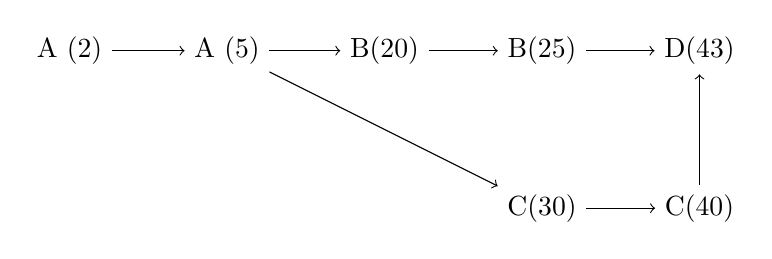
\begin{tikzpicture}
  [align=center,node distance=2cm]
  
  \node (1) {A (5)};
  \node (1o) [left of=1] {A (2)};
  \node (2a) [right of=1] {B(20)};
  \node (2b) [right of=2a] {B(25)};
  \node (3a) [below of=2b] {C(30)};
  \node (4) [right of=2b] {D(43)};
  \node (3b) [below of=4] {C(40)};
  
\draw [->] (1o) edge (1) (1) edge (2a) (2a) edge (2b) (2b) edge (4) (1) edge (3a) (3a) edge (3b) (3b) edge (4);
\end{tikzpicture}
\end{center}

Budeme rozlišovat \textit{město} a \textit{uzel - město v čase}. Budeme mít slovníkovou strukturu $cities$, která bude překládat názvy měst na objekty \textit{město}. Pokud budeme po $cities$ chtít doposud neexistující město, tak $cities$ takový objekt vytvoří. Slovník použijeme také pro dobu jízdy, kde pod klíčem \textit{Počátek}\#\textit{Klíč} budeme uchovávat číselnou hodnotu doby jízdy. Objekt \textit{město} bude obsahovat AVL strom z grafovými uzly (myšleno na mapě v čase). Mapové uzly jsou řazeny dle časů, které k nim náleží. Při procházení odjezdů budeme vytvářet hrany mezi mapovými uzly. Vyhledáme si první patřičné město a v daném AVL stromě hledáme uzel s konkrétním časem. Pokud existuje, tak tam vytvoříme hranu (s dalším, získaným podobně), pokud ne, tak na daném místě jej můžeme vytvořit, vybalancovat a přidat hranu. Pak ale nesmíme zapomenout, že kromě pohybu vlaky se lze pohybovat v čase i čekáním na nádraží. Stačí tedy projít každý AVL strom zleva doprava a pomocí následníků vytvářet hrany.
\\
Na konci stačí už na takový graf spustit třeba Dijkstrův algoritmus, který najde nejrychlejší cestu.
\pagebreak
\section{Pseudokód}
\begin{lstlisting}
# doby
doby = dic()
for i in range(m):
	from, to, time = input()
	dic[from + "#" + to] = time
	
# departures
cities = special_dic()
for i in range(r):
	from, to, departure = input()
	city_f = cities[from]
	city_t = cities[to]
	node_f = city_f.avl.get_create(departure)
	node_t = city_t.avl.get_create(departure+doby[from + "#" + to])
	node_f.add_edge(node_t)
	
# special
start, goal, start_time = input()
node_start = cities[start].avl.get_create(start_time)

# waiting
for city in cities:
	cur = city.avl.get_min()
	while next = city.avl.get_succ(cur):
		cur.add_edge(next)
		cur = next

output(spec_dijkstra(node_start, goal));
\end{lstlisting}

Upozorňuji, že operátor $[\hspace{0.2cm}]$ je v případě objektu $cities$ přetížený (vytváří, pokud neexistuje). Dále pak objektu $node\_start$ obsahuje tranzitivně odkaz ke zbytku grafu (pakliže je souvislý). Hrany mají váhy dle rozdílu času v uzlech (tj. každá hrana má přiřazený čas, který na ní strávíme). V tomto smyslu je definovaná funkce $w$

\section{Nejméně přestupů}
Podmínku co nejméně přestupů zajistíme tak, že si uvědomíme, jakým způsobem Dijkstra prohledává a vybírá hrany a vrcholy k relaxaci. Místo ukládání atributu vzdálenost od zdroje do každého vrcholu si můžeme ukládat dvojici (vzdálenost, počet navštívených hran) a při vybírání lepší cesty (relaxace) to zohlednit.
Tj. relax můžeme předefinovat zhruba na:
\begin{lstlisting}
relax(u, v, G):
	if (v.d > u.d + w(u,v)) or (v.d == u.d + w(u,v) and v.steps > u.steps + 1) :
		v.d = u.d + w(u, v)
		v.pred = u
		v.steps = u.steps + 1
\end{lstlisting}

Základní verzi to nepokazí, neboť úprava se týká pouze situací, kdy bychom si nepolepšili a doby by byly nerozhodně.

\section{Korektnost}
Pokud by existoval lepší způsob dopravy, tak by tomu musela odpovídat nějaká cesta uvnitř našeho komplexního grafu, neboť ten zahrnuje všechny cesty vlakem a všechny možné čekání. Taková cesta by ale byla nejkratší - dorazila by do cíle v nejkratším čase. Avšak na takový graf jsme pustili Dijkstrův algoritmus, takže tu stejnou cestu musí najít též, pokud existuje. Zároveň pakliže je nejlepší, že tak algoritmus lepší nenajde a najde právě tu. Nejméně přestupů bylo argumentováno o odstavec výš.

\section{Složitost}
Postavení slovníku trvání jízd trvá $O(m)$, neboť hashování názvů měst můžeme považovat za konstantní záležitost (omezení z reálného života). V pamětí zabere $O(m)$. Dále vybudování základního grafu mezi městy za pomocí odjezdů a příjezdů trvá $O(\textit{ř} \cdot \log(\textit{ř}))$ (logaritmus pochází z vyhledávání a vkládání do AVL stromu). V nejhorším případě se vytvoří pokaždé nový mapový uzel v co největším stromě (velikost lineárně \textit{ř}). V paměti to bude zabírat $O(\textit{ř})$, neboť nejhůře ř-krát provedeme do nějakého stromu insert. Zároveň jsme zde vytvořili právě \textit{ř} hran. Výsledkem je tedy graf o nejhůře \textit{ř} hranách a \textit{ř} vrcholech.

Pro čekání na nádraží musíme projít každý strom právě jednou a přidat ke každému uzlu patřičnou hranu na svého následovníka. To trvá $O(\textit{ř})$ a vytváříme zhruba \textit{ř} hran. Na výsledný graf o nejhůře \textit{ř} hranách a \textit{ř} vrcholech spouštíme jen lehce upraveného Dijkstru, což je $(\textit{ř} \cdot \log(\textit{ř}))$ (implementace za pomocí Fibonacciho haldy/rozumných sebevyvažovacích stromů).

Celkově jsme zabrali $O(\textit{ř}+m)$ paměti a $O(\textit{ř}\cdot \log(\textit{ř}) + m)$ času, kde $\textit{ř}$ je počet vlakových cest a $m$ počet dvojic, mezi kterými vlak jede.


\section{Mezistanice}
Pokud by vlaky zastavovaly v mezistanicích, tak si to můžeme představit tak, že jeden vlak do stanice přijede, kde skončí a vzápětí odjede ze stejné stanice nový vlak. Z uzlu budou tedy vést jak čekací hrana na stejné nádraží v budoucím čase, tak i hrana \textit{pokračujícího} vlaku. Nyní už počet řádků odjezdu není totožný s počtem vlakových cest, avšak pokud $\textit{ř}$ bude značit počet vlakových cest, tak je složitost stejná.

Tento přístup však narušuje integritu pro řešení nejmenšího počtu přestupů. Toho lze však docílit tak, že se v relaxu podíváme, zdali jsme nepřijeli stejným vlakem. To poznáme tak, že každá vlaková hrana bude mít přiřazeno \textit{id}, což může být dost dobře pořadí vlaku na vstupu a to budeme jednoduše porovnávat. Čekací hrany mohou mít všechny \textit{id = -1}, takže pokud budeme budeme cestovat: \textit{Otrokovice 12:20 $\rightarrow$ Otrokovice 12:35 $\rightarrow$ Otrokovice 13:01}, tak se nám počítadlo přestupů nezvětší, neboť tato podmínka je ošetřena. Úprava by mohla vypadat následovně:

\begin{lstlisting}
relax(u, v, G):
	if (v.d > u.d + w(u,v)) or (v.d == u.d + w(u,v) and v.steps > u.steps + 1) :
		v.d = u.d + w(u, v)
		v.pred = u
		# not a station and not the same train
		if (id(u, v) != -1 and id(u, v) != id(v. v.p):
			v.steps = u.steps + 1
\end{lstlisting}

\section{Alternativní řešení}
Úlohu by šlo řešit i modifikováním Dijkstry. Graf byl obyčejný (sestavený z tabulky doby jízdy) a hrany by u každého města byly v AVL stromu, takže by se pro daný čas dalo zjistit, jaké vlaky mají ještě odjet (nalezne se nejmenší větší než aktuální čas a pak se projdou následníci). Každé město by též u sebe mělo čas, v kolik se do něj dá nejdříve dostat.

Popsaný graf by však mohl být multigraf (není zaručeno, že mezi dvěma městy nejede stejným směrem dva a více vlaků). Na multigrafech klasický Dijkstra nefunguje a bylo by třeba jej ještě dál upravit.


\end{document}